\documentclass{article}
\usepackage[margin=1in]{geometry}
\usepackage[linesnumbered,ruled,vlined]{algorithm2e}
\usepackage{amsfonts}
\usepackage{amsmath}
\usepackage{amssymb}
\usepackage{amsthm}
\usepackage{enumitem}
\usepackage{fancyhdr}
\usepackage{hyperref}
\usepackage{minted}
\usepackage{multicol}
\usepackage{pdfpages}
\usepackage{standalone}
\usepackage[many]{tcolorbox}
\usepackage{tikz-cd}
\usepackage{transparent}
\usepackage{xcolor}
% \tcbuselibrary{minted}

\author{Nathan Solomon}

\newcommand{\fig}[1]{
    \begin{center}
        \includegraphics[width=\textwidth]{#1}
    \end{center}
}

% Math commands
\renewcommand{\d}{\mathrm{d}}
\DeclareMathOperator{\id}{id}
\DeclareMathOperator{\im}{im}
\DeclareMathOperator{\proj}{proj}
\DeclareMathOperator{\Span}{span}
\DeclareMathOperator{\Tr}{Tr}
\DeclareMathOperator{\tr}{tr}
\DeclareMathOperator{\ad}{ad}
\DeclareMathOperator{\ord}{ord}
%%%%%%%%%%%%%%% \DeclareMathOperator{\sgn}{sgn}
\DeclareMathOperator{\Aut}{Aut}
\DeclareMathOperator{\Inn}{Inn}
\DeclareMathOperator{\Out}{Out}
\DeclareMathOperator{\stab}{stab}

\newcommand{\N}{\ensuremath{\mathbb{N}}}
\newcommand{\Z}{\ensuremath{\mathbb{Z}}}
\newcommand{\Q}{\ensuremath{\mathbb{Q}}}
\newcommand{\R}{\ensuremath{\mathbb{R}}}
\newcommand{\C}{\ensuremath{\mathbb{C}}}
\renewcommand{\H}{\ensuremath{\mathbb{H}}}
\newcommand{\F}{\ensuremath{\mathbb{F}}}

\newcommand{\E}{\ensuremath{\mathbb{E}}}
\renewcommand{\P}{\ensuremath{\mathbb{P}}}

\newcommand{\es}{\ensuremath{\varnothing}}
\newcommand{\inv}{\ensuremath{^{-1}}}
\newcommand{\eps}{\ensuremath{\varepsilon}}
\newcommand{\del}{\ensuremath{\partial}}
\renewcommand{\a}{\ensuremath{\alpha}}

\newcommand{\abs}[1]{\ensuremath{\left\lvert #1 \right\rvert}}
\newcommand{\norm}[1]{\ensuremath{\left\lVert #1\right\rVert}}
\newcommand{\mean}[1]{\ensuremath{\left\langle #1 \right\rangle}}
\newcommand{\floor}[1]{\ensuremath{\left\lfloor #1 \right\rfloor}}
\newcommand{\ceil}[1]{\ensuremath{\left\lceil #1 \right\rceil}}
\newcommand{\bra}[1]{\ensuremath{\left\langle #1 \right\rvert}}
\newcommand{\ket}[1]{\ensuremath{\left\lvert #1 \right\rangle}}
\newcommand{\braket}[2]{\ensuremath{\left.\left\langle #1\right\vert #2 \right\rangle}}

\newcommand{\catname}[1]{{\normalfont\textbf{#1}}}

\newcommand{\up}{\ensuremath{\uparrow}}
\newcommand{\down}{\ensuremath{\downarrow}}

% Custom environments
\newtheorem{thm}{Theorem}[section]

\definecolor{probBackgroundColor}{RGB}{250,240,240}
\definecolor{probAccentColor}{RGB}{140,40,0}
\newenvironment{prob}{
    \stepcounter{thm}
    \begin{tcolorbox}[
        boxrule=1pt,
        sharp corners,
        colback=probBackgroundColor,
        colframe=probAccentColor,
        borderline west={4pt}{0pt}{probAccentColor},
        breakable
    ]
    \color{probAccentColor}\textbf{Problem \thethm.} \color{black}
} {
    \end{tcolorbox}
}

\definecolor{exampleBackgroundColor}{RGB}{212,232,246}
\newenvironment{example}{
    \stepcounter{thm}
    \begin{tcolorbox}[
      boxrule=1pt,
      sharp corners,
      colback=exampleBackgroundColor,
      breakable
    ]
    \textbf{Example \thethm.}
} {
    \end{tcolorbox}
}

\definecolor{propBackgroundColor}{RGB}{255,245,220}
\definecolor{propAccentColor}{RGB}{150,100,0}
\newenvironment{prop}{
    \stepcounter{thm}
    \begin{tcolorbox}[
        boxrule=1pt,
        sharp corners,
        colback=propBackgroundColor,
        colframe=propAccentColor,
        breakable
    ]
    \color{propAccentColor}\textbf{Proposition \thethm. }\color{black}
} {
    \end{tcolorbox}
}

\definecolor{thmBackgroundColor}{RGB}{235,225,245}
\definecolor{thmAccentColor}{RGB}{50,0,100}
\renewenvironment{thm}{
    \stepcounter{thm}
    \begin{tcolorbox}[
        boxrule=1pt,
        sharp corners,
        colback=thmBackgroundColor,
        colframe=thmAccentColor,
        breakable
    ]
    \color{thmAccentColor}\textbf{Theorem \thethm. }\color{black}
} {
    \end{tcolorbox}
}

\definecolor{corBackgroundColor}{RGB}{240,250,250}
\definecolor{corAccentColor}{RGB}{50,100,100}
\newenvironment{cor}{
    \stepcounter{thm}
    \begin{tcolorbox}[
        enhanced,
        boxrule=0pt,
        frame hidden,
        sharp corners,
        colback=corBackgroundColor,
        borderline west={4pt}{0pt}{corAccentColor},
        breakable
    ]
    \color{corAccentColor}\textbf{Corollary \thethm. }\color{black}
} {
    \end{tcolorbox}
}

\definecolor{lemBackgroundColor}{RGB}{255,245,235}
\definecolor{lemAccentColor}{RGB}{250,125,0}
\newenvironment{lem}{
    \stepcounter{thm}
    \begin{tcolorbox}[
        enhanced,
        boxrule=0pt,
        frame hidden,
        sharp corners,
        colback=lemBackgroundColor,
        borderline west={4pt}{0pt}{lemAccentColor},
        breakable
    ]
    \color{lemAccentColor}\textbf{Lemma \thethm. }\color{black}
} {
    \end{tcolorbox}
}

\definecolor{proofBackgroundColor}{RGB}{255,255,255}
\definecolor{proofAccentColor}{RGB}{80,80,80}
\renewenvironment{proof}{
    \begin{tcolorbox}[
        enhanced,
        boxrule=1pt,
        sharp corners,
        colback=proofBackgroundColor,
        colframe=proofAccentColor,
        borderline west={4pt}{0pt}{proofAccentColor},
        breakable
    ]
    \color{proofAccentColor}\emph{\textbf{Proof. }}\color{black}
} {
    \qed \end{tcolorbox}
}

\definecolor{noteBackgroundColor}{RGB}{240,250,240}
\definecolor{noteAccentColor}{RGB}{30,130,30}
\newenvironment{note}{
    \begin{tcolorbox}[
        enhanced,
        boxrule=0pt,
        frame hidden,
        sharp corners,
        colback=noteBackgroundColor,
        borderline west={4pt}{0pt}{noteAccentColor},
        breakable
    ]
    \color{noteAccentColor}\textbf{Note. }\color{black}
} {
    \end{tcolorbox}
}


\fancyhf{}
\setlength{\headheight}{24pt}

\date{\today}
\title{Physics 105B Lecture Notes, Fall 2024}

\begin{document}
\maketitle

The class textbook is \textit{Classical Mechanics of Particles and Systems, 5th edition} by Marion \& Thornton. These notes are a supplement for the textbook, not a replacement, so I won't cover everything from the course.
\begin{itemize}
    \item For midterm 1, study chapters 4, 9, 10
    \item For midterm 2, study chapters 4, 9, 10, 11, 12
    \item For the final, study chapters 4, 9, 10, 11, 12, \dots
\end{itemize}

\tableofcontents
\section{Review of Lagrangian mechanics (physics 105A)}
\subsection{Calculus of variations}
Use catenary and brachiostrome as examples
\subsection{Least action principle}
\subsection{Generalized momenta}
\subsection{Lagrange multipliers, forces from constraints}

\section{Phase diagrams}
For lots of systems, the state can be described by generalized positions ($q_1, q_2, \dots$) and generalized velocities ($\dot{q_1}, \dot{q_2}, \dots$). For example, the state of a pendulum at any time can be described by the vector
\[ \begin{bmatrix}
    \theta \\
    \dot{\theta}
\end{bmatrix}, \]
and if we know the state, we can calculate the rate of change of the state. That is,
\[ \begin{bmatrix}
    \dot{\theta} \\
    \ddot{\theta}
\end{bmatrix} \]
is a function of the state. We can visualize this as a vector field, where $x = \theta$ and $y = \dot{\theta}$. One amazing tool for animating vector fields is
\url{https://anvaka.github.io/fieldplay/}
\par
For the pendulum example, copy this code:
\begin{lstlisting}[language=C,frame=single]
// p.x and p.y are current coordinates
// v.x and v.y is a velocity at point p
vec2 get_velocity(vec2 p) {
  vec2 v = vec2(0., 0.);
  v.x = p.y;
  v.y = cos(p.x);
  return v;
}
\end{lstlisting}
\fig{pendulum.png}

For a Van der Pol oscillator, copy in this code, and experiment with changing $\mu$ (mu):
\begin{lstlisting}[language=C,frame=single]
float mu = 1.;
vec2 get_velocity(vec2 p) {
  return vec2(p.y, mu*(1.-p.x*p.x)*p.y-p.x);
}
\end{lstlisting}
Here is a Van der Pol oscillator with $\mu = 1$:
\fig{VanDerPol.png}

\section{Rotating reference frames}
Chapter 10 in the textbook. Copy example 10.5 (Foucault pendulum) to these notes

\section{Moment of inertia tensor}
If a system of particles is moving, and some point which we will call the origin is moving with velocity $V$, and $r_\alpha$ is the vector from the origin to some particle $\alpha$, and that particle is rotating about the origin with angular velocity $\omega$, then the velocity of that particle is $v_\alpha = V + \omega \times r_\alpha$. The kinetic energy of particle $\alpha$ is $m_\alpha v_\alpha^2 / 2$, and if you sum that over each $\alpha$, then we will see that the total kinetic energy is $T_{trans} + T_{rot}$, where $T_{trans} = (\sum_\alpha m_\alpha) V^2/2$ and $T_{rot} = \sum_\alpha m_\alpha (\omega \times r_\alpha)^2 / 2$. It makes sense to choose the origin to be the center of the mass, which minimizes $T_{rot}$ (assuming $\omega$ is the same for each particle). The rotational kinetic energy can also be written as
\[ T_{rot} = \frac{1}{2} \sum_{i,j} I_{i,j}\omega_i \omega_j \]
where $i,j \in \left\{ x, y, z \right\}$ and $I_{i,j}$ is the inertia tensor, defined as
\[ I_{i,j} := \sum_\alpha m_\alpha \left( \left( \delta_{i,j} \sum_k x_{\alpha,k}^2 \right) - x_{\alpha,i}x_{\alpha,j} \right)  \]
The diagonal elements of this matrix (I know it's a tensor, but I'm gonna call it a matrix anyway) are called moments of inertia, and the off-diagonal elements are called products of inertia.
\par
Note that if a mass distribution just lies along the $x$ axis, then $I_{y,y}=I_{z,z} > 0$ and the other 7 entries are all zero, which makes sense because that mass distribution is hardest to rotate about the $y$ axis and about the $z$ axis. If the formula for the off-diagonal entries resembles the formula for Pearson's correlation coefficient, which makes sense because ignoring some normalization factors, $r$ measures how much data lies along the line $y= \pm x$, and the products of inertia also measure how much mass lies along diagonal lines like $y=x,z=0$ and $z=y,x=0$ and $x=z, y=0$.
\par
Also note that $I$ is a symmetric matrix, so we can choose an orthonormal basis of eigenvectors (with real eigenvalues), and $I$ is diagonal in that basis. Those eigenvectors are called principle axes of inertia, and the eigenvectors are called the principle moments of inertia. If all three principle moments of inertia are the same, we call the body a spherical top, if two are the same but the other is different, we call it a symmetric top, and if all three are different, we call it an asymmetric top.
\par
If we're working with a continuous mass distribution, the formula becomes
\[ I_{i,j} = \int_{r \in \R^3} \rho(r) \left( \delta_{i,j} \sum_k x_k^2 - x_i x_j \right) \d^3r. \]
If we are working in a reference frame where $a$ is the position of the center of mass and the position of each particle is $R=a+r$ (and the components of that are $X_i=a_i+x_i$), and we let $M:= \sum_\alpha m_\alpha$ denote the total mass, then the inertia tensor in the center of mass frame is
\[ I_{i,j} = J_{i,j} - M \left( a^2 \delta_{i,j} - a_i a_j \right), \]
where $J$ is the inertia tensor in the lab frame. In fact, we don't need $a$ to be the center of mass, we just need $J$ to be the original inertia tensor and $I$ to be the inertia tensor in the frame centered at $a$. This equation is called Steiner's parallel-axis theorem. It clearly shows that rotational inertia about every axis is minimized iff you are in the COM frame.

\subsection{Angular momentum}
The momentum of each particle in our system is $p_\alpha = m_\alpha \omega \times r_\alpha$, so the angular momentum of the whole system is $L := \sum_\alpha r_\alpha \times p = \sum_\alpha m_\alpha r_\alpha \times (\omega \times r_\alpha)$. Using the vector identity $A \times (B \times A) = A^2B-A(A\cdot B)$, this becomes
\[ L = \sum_\alpha m_\alpha \left( r_\alpha^2 - r_\alpha (r_\alpha \cdot \omega) \right). \]
Each component of $L$ can be written as
\[ L_i = \sum_j I_{i,j} \omega_j. \]
so $L = I \cdot \omega$.
\par
The time derivative of $L$ is the net torque on the body, $\dot{L} = N := \sum \tau$. The rotational kinetic energy is $T_{rot} = \omega \cdot L / 2$.

\subsection{Stress tensor}
A lot of your intuition for the moment of inertial tensor can be applied to the stress tensor $\sigma$, which is another contravariant, symmetric, second-order tensor. It represents the forces on each point in a material. Thinking of it as a 3 by 3 matrix, the diagonal elements represent the tensile stress along each axis. So for example, $\sigma_{1,1}$ would be positive if the material it being stretched along the $x$ axis at that point, and negative if it is being squished along the $x$ axis at that point.
\par
The off-diagonal elements of $\sigma$ represent shear forces. For example, if $\sigma_{1,2} = \sigma_{2,1} > 0$, then there is some shearing force in the $x,y$ plane. Such a force could also be treated as a pulling force in the direction of the unit vector $\pm \frac{1}{\sqrt{2}} (\hat{x} + \hat{y})$. By treating all of the shearing forces as pulling or squishing along some axis other than $\hat{x}$, $\hat{y}$, or $\hat{z}$, we can describe the stress tensor with just the tensile stress along those 3 axes, which we can ensure are orthogonal, because $\sigma$ is symmetric. This is equivalent to diagonalizing the stress tensor.
\par
To intuitively understand these off-diagonal elements, imagine a square pice of sheet metal lying in the $x,y$ plane, with one edge flushed to the $x$ axis and another flushed to the $y$ axis. Then apply a shear force $F \propto y \hat{x}$ to it, which points along the $x$ axis and is proportional to the $y$ coordinate. This force acts to stretch the square into a rhombus, effectively pulling (that is, applying tensile stress) in the $\frac{1}{\sqrt{2}} (\hat{x} + \hat{y})$ direction.
\par
Stress has units of force per area. One Pascal is a Newton per meter squared, and one atmosphere is about $101.3$ kilopascals. If the stress tensor is some scalar $\sigma_{1,1}$ times the identity tensor, then we can say that the pressure is $-\sigma_{1,1}$. Air pressure at sea level is very close to 1 atm, and air pressure pretty much decays exponentially with altitude.
\begin{center}
    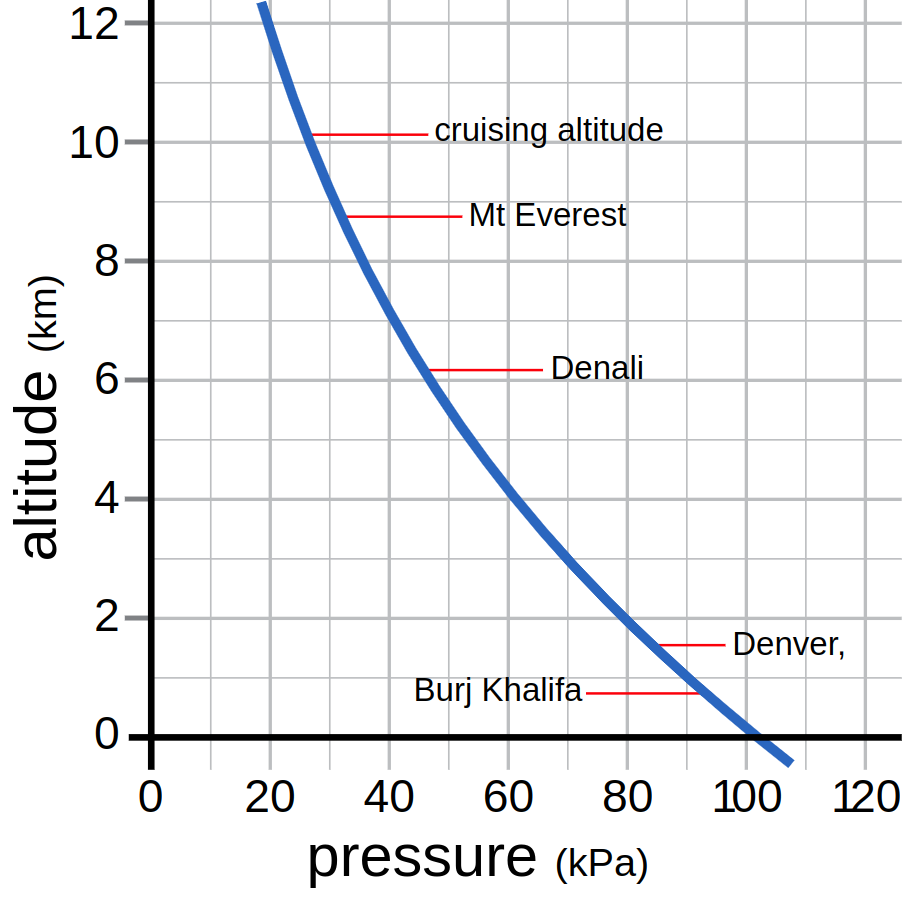
\includegraphics[width=0.5\textwidth]{pressure.png}
\end{center}

\section{Euler angles}
For this section, I will call my axes $x_1$, $x_2$, and $x_3$ instead of $x$, $y$, and $z$.
\par
Any rotation in 3D space can be decomposed into these three steps (in order):
\begin{itemize}
    \item Rotate by an angle $\phi$ around the $x_3'$ axis. Note that this will move the $x_1'$ and $x_2'$ axes. The axes of the new system are now called $x_1'', x_2'', x_3''$.
    \item Rotate by an angle $\theta$ about the new $x_1''$ axis (which will change the directions of the $x_2''$ and $x_3''$ axes). The axes of the system after this rotation are called $x_1''', x_2''', x_3'''$.
    \item Rotate by an angle $\psi$ about the newest $x_3'''$ axis. After all 3 of these rotations are done, call the transformed axes $x_1, x_2, x_3$.
\end{itemize}
Call those rotations $\lambda_\phi$, $\lambda_\theta$, and $\lambda_\psi$, respectively. Their composition, $\lambda=\lambda_\psi \lambda_\theta \lambda_\phi$, will map a vector $x'$ to a vector $x$.
\[ \lambda_\phi = \begin{bmatrix}
    \cos \phi & \sin \phi & 0 \\
    -\sin \phi & \cos \phi & 0 \\
    0 & 0 & 1
\end{bmatrix}, \lambda_\theta = \begin{bmatrix}
    1 & 0 & 0 \\
    0 & \cos \theta & \sin \theta \\
    0 & -\sin \theta & \cos \theta
\end{bmatrix}, \lambda_\psi = \begin{bmatrix}
    \cos \psi & \sin \psi & 0 \\
    -\sin \psi & \cos \psi & 0 \\
    0 & 0 & 1
\end{bmatrix}. \]
\[ x = \lambda_\psi x''', x''' = \lambda_\theta x'', x'' = \lambda_\phi x'. \]
If we define $\omega_\phi = \dot{\phi}, \omega_\theta = \dot{\theta}, \omega_\psi=\dot{\psi}$, then observe that $\dot{phi}$ points along the fixed $x_3'$ axis, $\dot{\theta}$ points along the line of nodes -- that is, the line formed by the intersection of the $x_1,x_2$ plane and the $x_1',x_2'$ plane -- and $\dot{\psi}$ points along body's $x_3$ axis.
\fig{Euler angles.png}
\begin{align*}
    \omega_1 &= \dot{\phi}_1 + \dot{\theta}_1 + \dot{\psi}_1 = \dot{\phi} \sin \theta \sin \psi + \dot{\theta} \cos \psi \\
    \omega_2 &= \dot{\phi}_2 + \dot{\theta}_2 + \dot{\psi}_2 = \dot{\phi} \sin \theta \cos \psi - \dot{\theta} \sin \psi \\
    \omega_3 &= \dot{\phi}_3 + \dot{\theta}_3 + \dot{\psi}_3 = \dot{\phi} \cos \theta + \dot{\psi}.
\end{align*}
If we let the body axes $x_1, x_2, x_3$ be the principal axes of a rigid body, then treating the Eulerian angles $\phi, \theta, \psi$ as generalized coordinates and plugging them into the Euler-Lagrange equation gives us the Euler equations:
\begin{align*}
    (I_2-I_3)\omega_2\omega_3 - I_1 \dot{\omega_1} &= 0 \\
    (I_3-I_1)\omega_3\omega_1 - I_2 \dot{\omega_2} &= 0 \\
    (I_1-I_2)\omega_1\omega_2 - I_3 \dot{\omega_3} &= 0.
\end{align*}

\section{Coupled oscillators (chapter 12)}
If you have a bunch of atoms in a crystal, and you look at a one dimensional piece of it (along the right axis), it will look like a bunch of atoms in a line, each one bonded to its two neighbors. We can treat this as a bunch of masses joined by massless springs. This system is not chaotic, because the differential equation for the positions of each mass is linear. Instead of representing the state of the system by describing the position of each atom, we can change basis, and represent it in terms of normal modes, The dimension of the state space doesn't change -- if we had $n$ degrees of freedom before changing basis (we could say there are $n/d$ masses which are free to move in $d$ dimensions), there will be $n$ normal modes.

\end{document}
